\chapter{State of the Art} \label{chapter:state_of_the_art}
There are several hypervisors that have been developed in the last few years, as well as SDN controllers. We will now consider the benefits and drawbacks of each alternative and, at the end of the chapter, explain the rationale behind the ones we will end up using. 

Regarding the hypervisors, some, if not most, of them are not really usable in the present day, i.e., they are only a prototype or a proof of concept. They will be mentioned regardless for the sake of completeness.

\section{Hypervisor Candidates}
For each entry, we will avoid the implementation and technical details. The point of this section is to offer a fairly simple overview for each hypervisor, with just enough details so that we can make a decision on whether to use it or not.

\subsection{CoVisor}
CoVisor is defined as "A new kind of network hypervisor that enables, in a single network, the deployment of multiple control applications written in different programming languages and operating on different controller platforms"\cite{covisor}.

CoVisor's main selling point is its flexibility, it is intended to allow different technologies to work together in order to create a "best of breed" network, as its authors call it. They also have a strong consideration for efficiency, as they mention how to exploit new efficient algorithms.

While CoVisor seems like a valid choice, it presents two problems for this project in particular.
\begin{itemize}
    \item Adds unnecessary complexity. We are looking for a simple hypervisor that will allow us to slice a network. CoVisor does this, but it is designed for handling many different controllers at once, which gets very complex very fast.
    \item It is nothing more than a proof of concept. There is no code available that we can use to test it, at least not at the time of writing this document.
\end{itemize}

\subsection{FlowVisor}
Flowvisor is a hypervisor developed at Standford University. It is also fairly simple. It creates different slices which correspond to different controllers and relays the packets accordingly. Flowvisor is also open source and there are some good examples about network slicing available online.

Flowvisor looks like a good candidate for the project, but it has a few drawbacks.
\begin{itemize}
    \item Despite being open source, it has not been updated since 2013.
    \item It only works with OpenFlow 1.0.
    \item It definitely lacks some proper documentation about its features and implementation details.
    \item The slices are restricted to a subset of the physical topology.
\end{itemize}

The fact that FlowVisor has not been updated in years and the lack of documentation seem to be linked, as the code itself seems to work for the most part. It looks like FlowVisor is just lacking a cleaner API due to the absence of updates, aside from the OpenFlow version compatibility issue.

Regardless of these issues, FlowVisor is very widespread and is commonly used, probably due to the fact that is open source. This ensures that it has been tested thoroughly in many different topologies, thus improving its stability and minimizing possible bugs.

\subsection{VeRTIGO}
VeRTIGO stands for ViRtual TopologIes Generalization in Openflow networks \cite{vertigo}. It is presented as an extension to FlowVisor, aiming to overcome its limitations. One of these limitations, as mentioned by the authors of VeRTIGO, is the fact that the virtual topologies created by FlowVisor are just a subset of the physical topology.

The authors' idea is based on enhancing FlowVisor's "intelligence" in order to circumvent its limitations in slice creation and management, as well as increasing its robustness to network congestion and link failures. They also mention to have performed some testing in a real production environment.

Since VeRTIGO is presented as an extension to FlowVisor, it looks like a good choice. However, it seems like VeRTIGO never made it out of the prototype phase and it is not available for public use.

 \subsection{RadioVisor}
 As its name indicates, RadioVisor\cite{radiovisor} is a hypervisor designed around Radio Access Networks. The authors point out the current difficulties and cost of deploying basetations. They mention SoftRAN\cite{softran}, which is SDN technology applied to Radio Access Network, as an improvement over the situation. However, they argue that a better solution would be to extend SoftRAN and use RadioVisor to dynamically slice the network based on traffic and congestion. Unlike conventional hypervisors, RadioVisor also has to take into account the possible interferences between the different slices. Now, there are a few issues with this hypervisor.
\begin{itemize}
    \item Too specialized. We are looking for a more general purpose hypervisor that supports a broader array of networks.
    \item As with many other hypervisors in this chapter, we have been unable to find the source code or a functional version of it.
\end{itemize}

\subsection{AutoSlice}
AutoSlice\cite{autoslice} is slightly different from the rest of the hypervisors discussed in this chapter. It not only aims to provide slicing capabilities, its main goal is to automate such process. By relaying on automation, it would be possible to rent an SDN to different tenants while minimizing the need for manual intervention. This is made possible by giving each tenant the means to lease "programmable network slices", according to the authors. An overview of this architecture is shown in Figure \ref{fig:autoslice}.

\begin{figure}
  \centering
  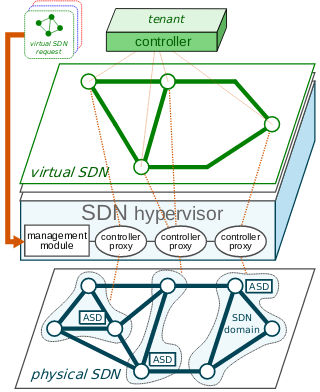
\includegraphics[width=0.6\linewidth]{imagenes/StateOfTheArt/AutoSlice_architecture.png}
  \caption[AutoSlice architecture.]{AutoSlice architecture\cite{autoslice}.}
  \label{fig:autoslice}
\end{figure}

One issue that arises when reading the article about AutoSlice, is that it has only been tested with OpenFlow 1.0. Ideally we would like to use a hypervisor that is capable of handling the latest version of OpenFlow, i.e, OpenFlow 1.5.

Regarding the viability of this hypervisor, it is too complex for what we are trying to do. But even if we wanted to use it, there is no code in sight. It seems like it was just a proof of concept. 

\subsection{ADVisor}
The authors of ADVisor\cite{advisor} refer to FlowVisor as a recent approach towards network virtualization. However, they also acknowledge its limitations when it comes to flowspace sharing and traffic interferences. They propose ADVisor (ADvanced Flowvisor) as a way to overcome those limitations. 

ADVisor is designed to extend FlowVisor in order to provide two additional virtualization functions: Virtual link management, and Virtual ports management. As a result, ADVisor is able to work with FlowVisor in a nested way, as shown in Figure \ref{fig:advisor}.

\begin{figure}
  \centering
  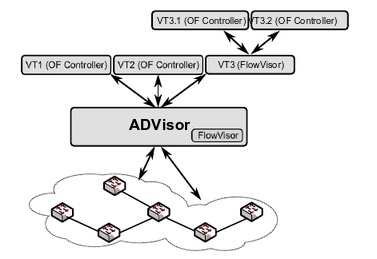
\includegraphics[width=0.8\linewidth]{imagenes/StateOfTheArt/ADvisor_architecture.png}
  \caption[ADVisor architecture.]{ADVisor architecture\cite{advisor}.}
  \label{fig:advisor}
\end{figure}

As for the possible drawbacks, ADVisor seems to slightly surpass the scope of this project. And, again, it appears to be just a proof of concept with no source code or binary files available for us to test it.

\section{OpenFlow Controllers}
This section will go through a quick overview of the most popular OpenFlow controllers, hoping to find the most suitable one for the project.

\subsection{NOX}
NOX was the first OpenFlow controller. Originally developed by Nicira Networks and then released to the research community back in 2008. According to its archived website\cite{nox}, NOX had the following features: 
\begin{itemize}
    \item C++ OpenFlow 1.0 API.
    \item Fast, asynchronous IO.
    \item Targeted at Ubuntu 11.10 and 12.04.
    \item Includes sample components: Topology discovery, learning switch and network-wide switch.
\end{itemize}

It is evident that NOX is heavily outdated and its use is not recommended. Nonetheless, it is featured in this chapter as it is the predecessor to another popular SDN controller, POX.

\subsection{POX}
While the last time POX was updated was two years ago, it is still much more recent than NOX. Although POX is considered the successor to NOX, POX's features differ considerably from NOX's.
\begin{itemize}
    \item Python 2.7 OpenFlow API.
    \item Supports pretty much anything that can run Python 2.7 (Windows, Mac OS, Linux, Android, FreeBSD, etc).
    \item Support for PyPy JIT compiler for a performance boost.
    \item It can only handle OpenFlow 1.0.
    \item Includes a wide variety of sample components.
\end{itemize}

Moreover, POX comes already bundled with the Mininet virtual machine, so it does not require any additional installation. 

\subsection{OpenDaylight Controller}
Founded in 2013, the OpenDaylight foundation develops a very popular open source SDN controller platform. They are also a member of the Linux Foundation Networking. They like to name each release after an element from the periodic table, the most recent one being Neon, which is their tenth release (Neon's atomic number is 10). OpenDaylight Neon is the most complex SDN controller featured in this section. For an overview of its architecture, see Figure \ref{fig:opendaylight}.

\begin{figure}
  \centering
  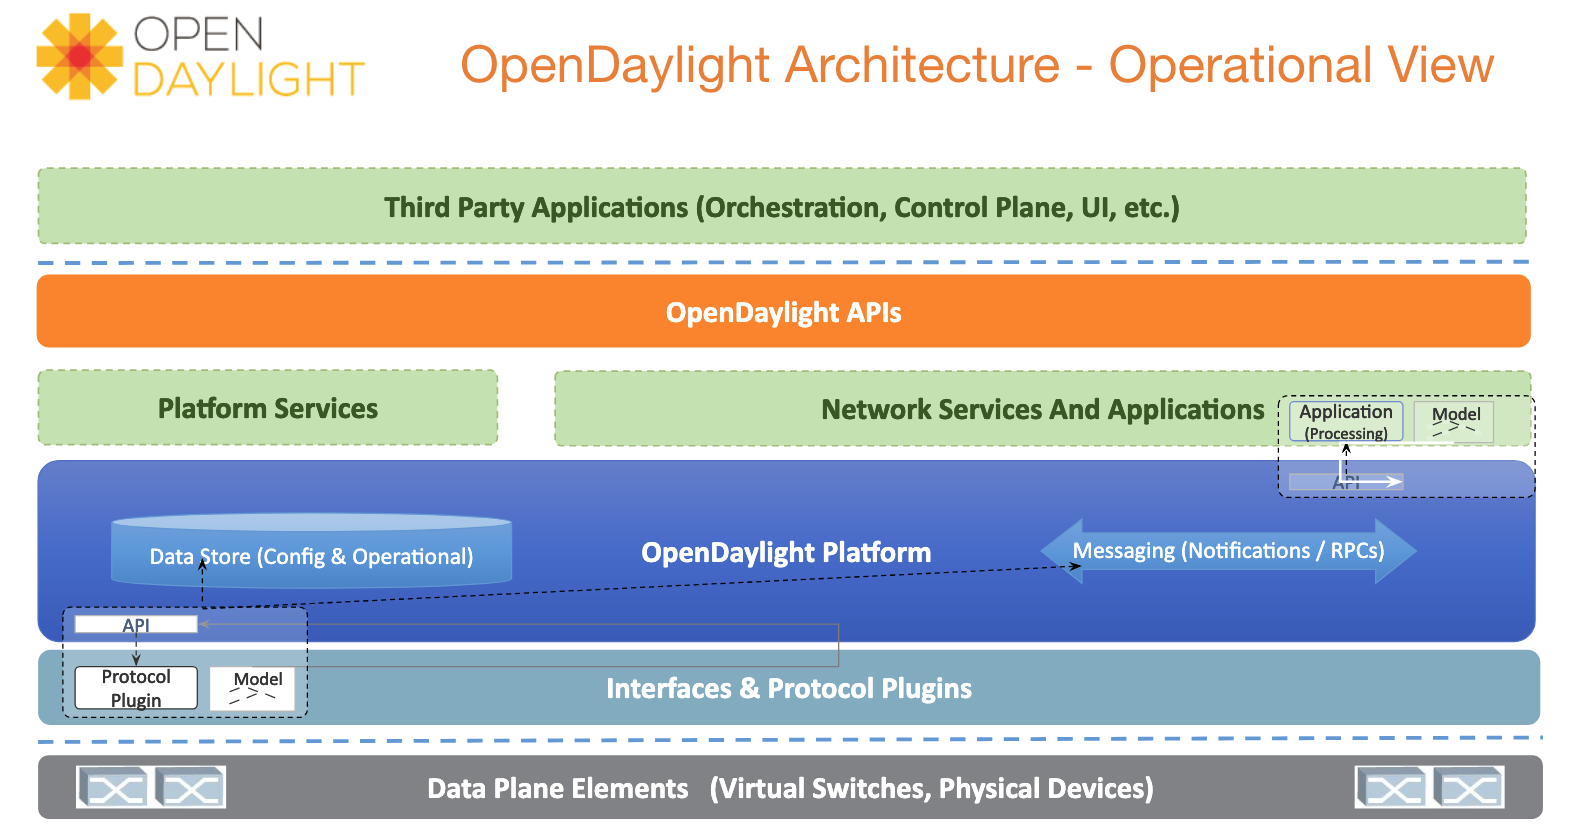
\includegraphics[width=0.8\linewidth]{imagenes/StateOfTheArt/open_daylight.png}
  \caption[OpenDaylight Neon architecture overview.]{OpenDaylight Neon architecture overview\cite{opendaylight}.}
  \label{fig:opendaylight}
\end{figure}

OpenDaylight main advantages are:
\begin{itemize}
    \item Thoroughly tested and production ready. Used by a lot of companies all over the world.
    \item Supported by big companies such as AT\&T, Cisco and Ericsson among others.
    \item Plenty of features from more than 100.000 commits, e.g, cloud network virtualization.
    \item Modular. Only install features you need.
    \item Graphical interface. Makes it more user friendly than terminal-only controllers.
    \item Good documentation.
\end{itemize}

OpenDaylight is a great controller. However, and despite being modular, it is quite heavier memory wise than the rest of alternatives. It is also written in Java, so a JRE is needed in order to run the OpenDaylight controller. 

\subsection{Beacon}
Developed at the Standford University in 2010, Beacon\cite{beacon} is an open source OpenFlow controller written in Java. Beacon was mostly designed with three goals in mind.
\begin{itemize}
    \item Developer Productivity.
    \item Runtime Modularity. The goal is to be able to start and stop applications while the controller itself is running.
    \item Performance. Multi thread implementation.
\end{itemize}

Beacon, like NOX, is quite outdated with its last update happening on May of 2011. Nevertheless, Beacon is an OpenFlow controller worth mentioning, as it is the base for another controller, Floodlight.

\subsection{Floodlight}
Floodlight started as fork of Beacon in 2011, therefore it is also open source. Unlike Beacon, Floodlight's last update, at the time of writing this document, was released on May of 2019. Floodlight's main strengths are:
\begin{itemize}
    \item Well tested.
    \item Good documentation.
    \item Includes sample components.
    \item Graphical interface.
    \item Supports OpenFlow from version 1.0 to 1.5.
    \item Modular.
    \item Multi threaded. 
    \item Can handle mix-OpenFlow and non OpenFlow networks.
\end{itemize}

In addition, despite Floodlight being written in Java, it can be extended using its REST API. In fact, its sample components use Python to access the REST API.

\section{Conclusions}
It is now time to make a decision and choose from the several options presented in this chapter. In regards to the OpenFlow controller, we could choose more than one since we intend to use multiple controllers. Because of the added complexity that using different controllers entails, we will just choose one. 

\subsection{Hypervisor}
Given that only one of the previous entries is a valid candidate, i.e., it is publicly available, it is trivial to make the choice, we will use FlowVisor. It has a few inconveniences, e.g., lack of proper documentation and limited version compatibility with OpenFlow. Nonetheless, FlowVisor should be sufficient to carry out the project.

There are some more hypervisors that have not been mentioned, yet none of them are publicly available at the time of writing this document.

It seems like the developing of hypervisors for network slicing/virtualization was a hot topic a few years ago, but either almost none of them made it past the proof of concept or they were completely privatized and used internally within the industry. Furthermore, the only one that made it to open source, i.e., FlowVisor, was pretty much abandoned for unknown reasons as its three contributors moved on to different projects.

\subsection{OpenFlow Controller}
The OpenFlow controller section is much more competitive than the hypervisor section. There are multiple good choices, each one with its pros and cons. In order to make the best decision, let us establish the baselines for what we want from a controller.
\begin{itemize}
    \item Simple and lightweight. The whole point of using a hypervisor is to simplify the logic of the controller.
    \item Python based. This is mainly a preference, as Python is the language we are most proficient at.
    \item No need to support OpenFlow higher than 1.0, since FlowVisor itself only supports OpenFlow 1.0.
    \item High performance is not a concern. The logic of the controller will be very simple.
    \item Well documented or includes sample components.
    \item A graphical interface is not necessary.
    \item Not extremely outdated.
\end{itemize}

Given these requirements, the controller that fits the most is the POX controller. POX is simple enough for what we need, lightweight, comes with sample modules, extendable with Python and, on top of that, it comes already installed with the Mininet Virtual Machine.
